\documentclass[final]{cvpr}

\usepackage{times}
\usepackage{epsfig}
\usepackage{graphicx}
\usepackage{amsmath}
\usepackage{amssymb}

% Include other packages here, before hyperref.

% If you comment hyperref and then uncomment it, you should delete
% egpaper.aux before re-running latex.  (Or just hit 'q' on the first latex
% run, let it finish, and you should be clear).
\usepackage[pagebackref=true,breaklinks=true,colorlinks,bookmarks=false]{hyperref}

%%%%%%%%% PAPER ID  - PLEASE UPDATE
% \def\cvprPaperID{****} % *** Enter the CVPR Paper ID here
%\def\httilde{\mbox{\tt\raisebox{-.5ex}{\symbol{126}}}}

\def\cvprPaperID{****} % *** Enter the CVPR Paper ID here
\def\confYear{CVPR 2024}

\begin{document}

%%%%%%%%% TITLE - PLEASE UPDATE
\title{Real and Fake Face Detection}  % **** Enter the paper title here

\author{J L\\
1234567\\
Master in Data and Computer Science\\
{\tt\small Person1@i1.org}
\and
X P\\
1234567\\
Master in Data and Computer Science\\
{\tt\small Person1@i2.org}
\and
R C\\
1234567\\
Master in Data and Computer Science\\
{\tt\small Person1@i2.org}
\and
H K \\
1234567\\
Master in Data and Computer Science\\
{\tt\small Person1@i2.org}
\and
Mentor: PLEASE DO NOT UPLOAD PERSONAL INFORMATION TO PUBLIC PLATFORM
}


\maketitle
\thispagestyle{empty}


%%%%%%%%% BODY TEXT - ENTER YOUR RESPONSE BELOW
\section{Abstract}

\section{Introduction}

In this project, our primary aim is to compile a comprehensive dataset consisting of genuine and altered human facial images. Subsequently, we seek to develop a convolutional neural network (CNN) capable of discerning fabricated images within this dataset. Our focus extends to evaluating the performance of our CNN model against established benchmarks, including the baseline ResNet model, MobileNetV2, and GramNet (with Gram Block). Through meticulous data collection and model development processes, we aim to provide insights into the efficacy of various CNN architectures for detecting manipulated images. Throughout model development, we experiment with various CNN architectures, exploring differences in depth, layer types, and regularization methods. We benchmark our CNN model against the baseline and other models using identical test datasets.

%------------------------------------------------------------------------
\section{Related Work}

\section{Method}
\subsection{Datasets WIP}
We adopt two different public datasets to train our model. The first dataset is a compact one with appropriate 1400 training images. The dataset contains expert-generated high-quality photoshopped face images, and images are composite of different faces, separated by eyes, nose, mouth, or whole face\cite{kaggledatasetRealAndFakeFaceDetection}.

The second dataset is a large-scale dataset with appropriate 190K images. This dataset contains both manipulated images and real images, manipulated images are faces are generated by multiple ways, each image is a 256 x 256 jpg image of human face either real or fake\cite{kaggledatadeepfakeandrealimages, le2021openforensics}.

Cross-datasets Training WIP

\subsubsection{Simple CNN}

A simple CNN network can be used to test the correctness of program exectution and observe the flow of data. Because of its brief structure, it can significantly reduce the cost of computing resources. At the same time, it can alos be used as one of the benchmark performance indicators for comparison and analysis with other types of subsequent network models.

This convolutional neural network is designed for image classificaion, structured with an input layer which taks 3-channel RGB images, followed by three convolutional layers, each with a 3x3 kernal and padding of 1, progressively increasing the number of filters from 32 to 64 and finally 128. Each convolutional layer is followed by a ReLU activation function and a 2x2 max pooling layer. The output is flattened and passed throught two fully connected layers. The first FC layer transforms the feature map into 512 features, followed by another ReLU, and the second FC layer reduces it to 2 outputs for classification. 

\subsubsection{Improved CNN}

The Improved CNN represents an enhancement of the previous 'SimpleCNN' model. it is designed to achieve better performance by adopting serveral architectural adjustments to increase the network's capacity and reduce overfitting.

Compared with the basic version of CNN, the improved version of convolutional neural network has been improved in the following aspects: An additional convolutional layer has been introduced; The depth is increased with 256 filters; Each convolutional layer is now followed by a batch normalization layer; A dropout layer with a rate is introduced before the first fully connected layer; Also an increased fully connected layer capacity, transforms the feature maps into a larger dimensional space.


\section{Experiments}

\subsection{Dataset 1 WIP}

Experienments start with the small-scale dataset 1, wiit simpleCNN structure, as in Figure~\ref*{fig:ex-d1-simplecnn-results}, after 20 rounds of iterations, the validation accuracy remains fluctuating within a range and has not increased significantly. The accuracy is about 60\%.

The ImprovedCNN brought slight better performance in the later iterations of training. As shown in Figure~\ref*{fig:ex-d1-improvedcnn-results}, the validation accuracy range came to between 60\% to 65\%, but it was very unobvious and thus did not bring significantly improvement.

\begin{figure}[t]
   \centering
   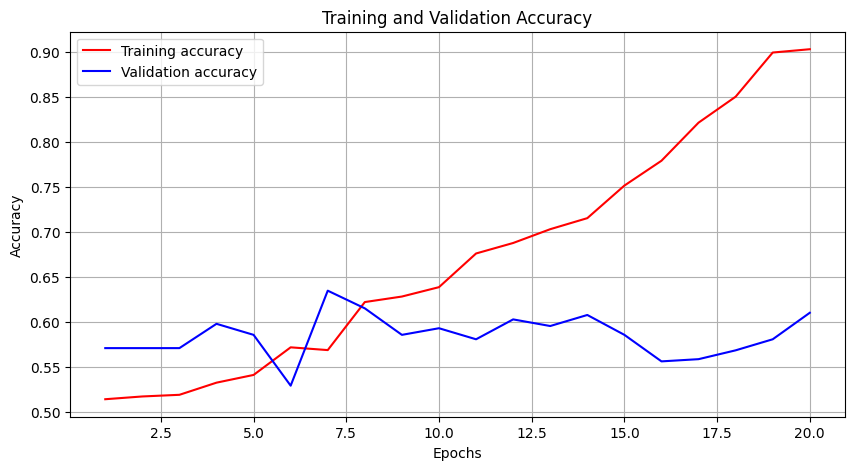
\includegraphics[width=0.9\linewidth]{img/ex-d1-simplecnn-accuracy-results.png}
   \caption{Training and Validation results of simple CNN with the compact dataset}
   \label{fig:ex-d1-simplecnn-results}
\end{figure}

\begin{figure}[t]
   \centering
   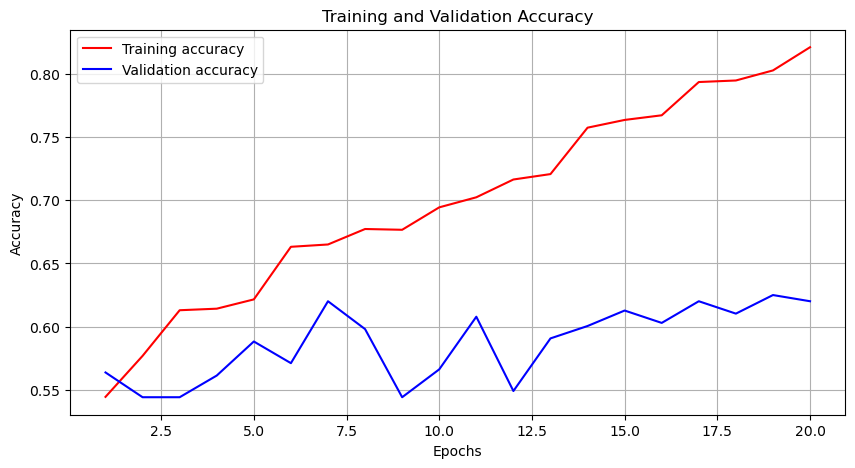
\includegraphics[width=0.9\linewidth]{img/ex-d1-improvedcnn-accuracy-results.png}
   \caption{Training and Validation results of improved CNN with the compact dataset}
   \label{fig:ex-d1-improvedcnn-results}
\end{figure}

% \begin{figure}[t]
%    \centering
%    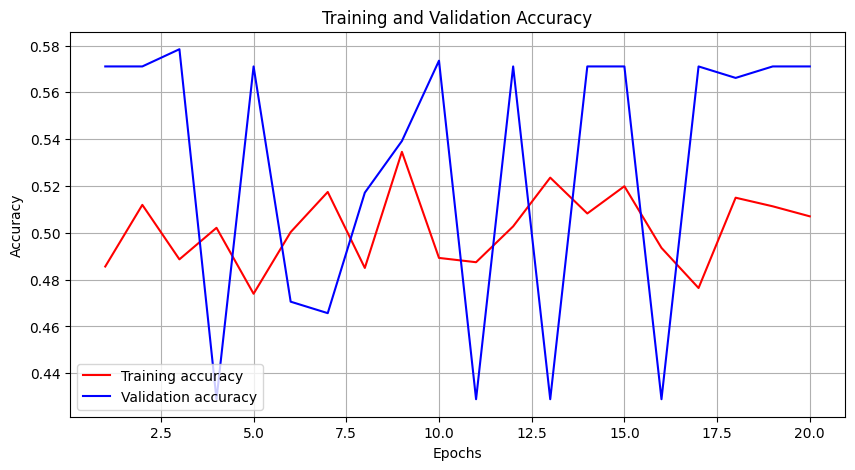
\includegraphics[width=0.9\linewidth]{img/ex-d1-gramnet51-accuracy-results.png}
%    \caption{Training and Validation results of GramNet51 with the compact dataset}
%    \label{fig:ex-d1-gramnet51-results}
% \end{figure}

% \begin{figure}[t]
%    \centering
%    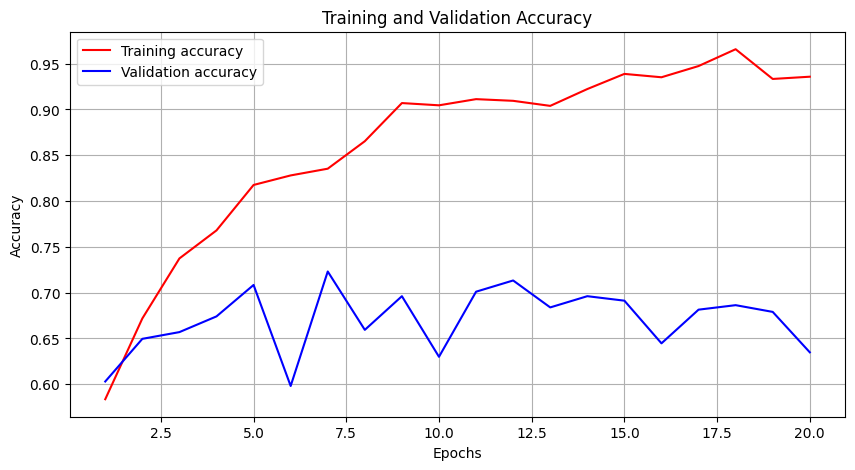
\includegraphics[width=0.9\linewidth]{img/ex-d1-MobileNetV2-accuracy-results.png}
%    \caption{Training and Validation results of MobileNetV2 with the compact dataset}
%    \label{fig:ex-d1-MobileNetV2-results}
% \end{figure}

\subsection{Dataset 2 WIP}

The situation changes when large-scale data sets are adopted. With the support of the training set of 140k+ images, even the network structure of simpleCNN has achieved a huge leap in verification accuracy. As shown in Figure~\ref*{fig:ex-d2-simplecnn-results}, it reached about 94\% after 20 rounds of iterations. Compared with the case of using the simplified data set (Figure~\ref*{fig:ex-d1-simplecnn-results}), an improvement of more than 30\% is achieved.

The performance of the improved CNN network structure in large-scale datasets is shown in Figure~\ref*{fig:ex-d2-improvedcnn-results}. Although it has been greatly improved, the advantage over simpleCNN is very little. after 20 epochs, it reached about 96\% validation accuracy.

\begin{figure}[t]
   \centering
   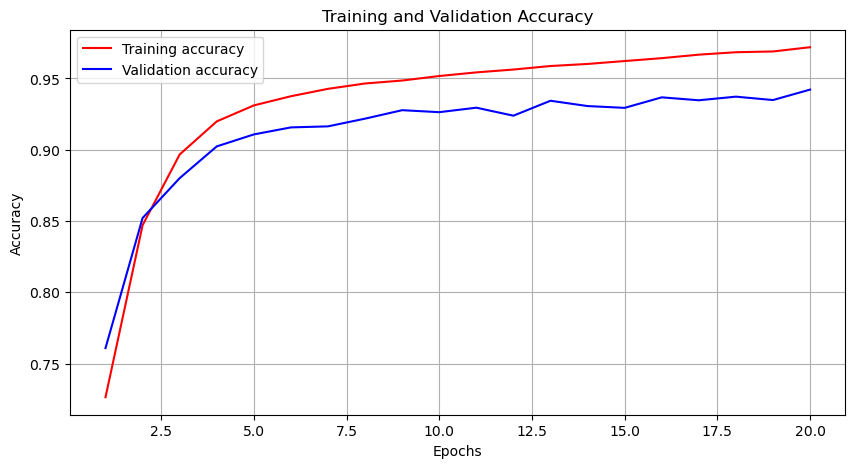
\includegraphics[width=0.9\linewidth]{img/ex-d2-simplecnn-accuracy-results.png}
   \caption{Training and Validation results of simple CNN with the large-scale dataset}
   \label{fig:ex-d2-simplecnn-results}
\end{figure}

\begin{figure}[t]
   \centering
   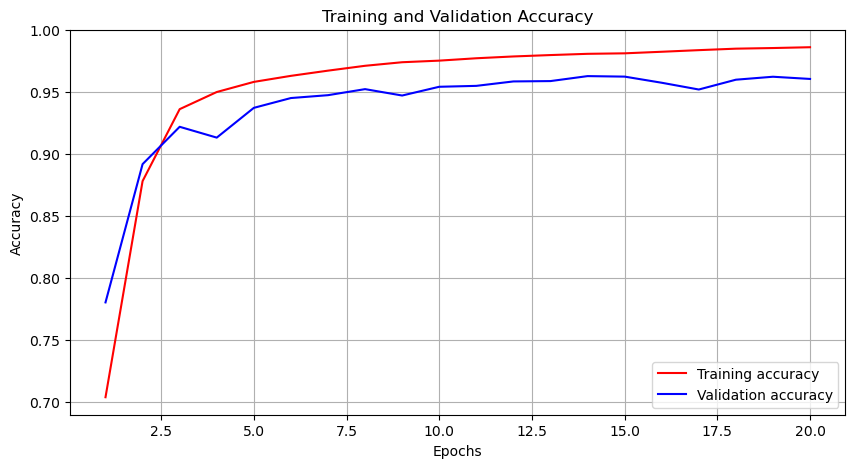
\includegraphics[width=0.9\linewidth]{img/ex-d2-improvedcnn-accuracy-results.png}
   \caption{Training and Validation results of improved CNN with the large-scale dataset}
   \label{fig:ex-d2-improvedcnn-results}
\end{figure}

% \begin{figure}[t]
%    \centering
%    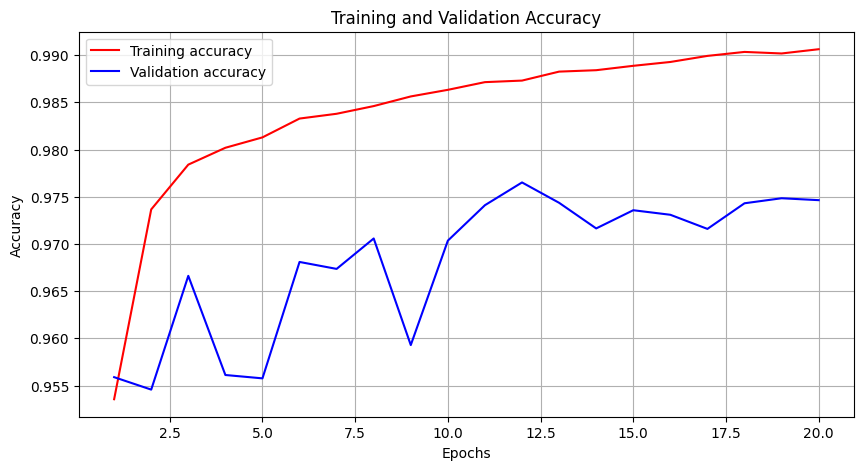
\includegraphics[width=0.9\linewidth]{img/ex-d2-mobilenetv2-accuracy-results.png}
%    \caption{Training and Validation results of MobileNetV2 with the large-scale dataset}
%    \label{fig:ex-d2-MobileNetV2-results}
% \end{figure}


\subsection{Cross-datasets Training WIP}

During the experiment and testing process, we found that the models trained on the two data sets can achieve better results when tested on their own data sets. However, when performing cross-testing, when testing on another data set, the performance was disappointing.

In order to achieve better generalization ability of the model, we adopted the cross-data training method.

An ImprovedCNN structure has no advantage in capturing and managing features from cross-datasets, as in Figure~\ref*{fig:ex-cd-improvedcnn-results}, the performance is quite poor in absolute terms, with only about 51\% accuracy. It is also very unstable in relative terms, thus it is basically unusable.

\begin{figure}[t]
   \centering
   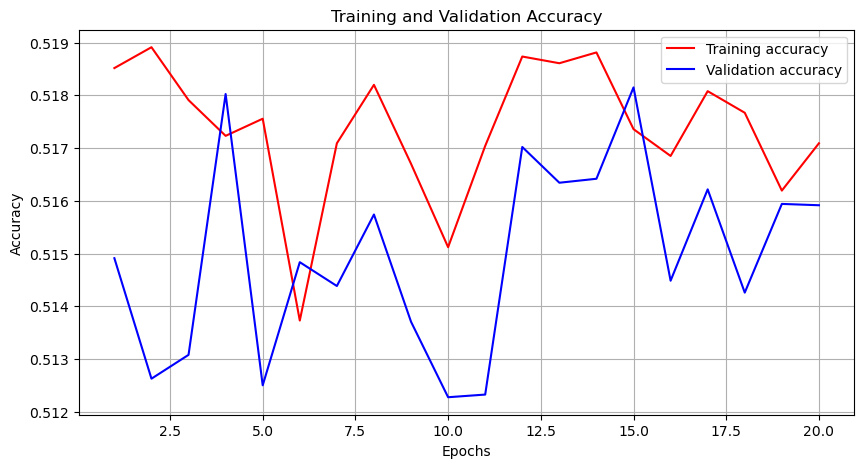
\includegraphics[width=0.9\linewidth]{img/ex-cd-improvedcnn-accuracy-results.png}
   \caption{Training and Validation results of improved CNN with the cross-datasets}
   \label{fig:ex-cd-improvedcnn-results}
\end{figure}

WIP

\subsection{Dataset generated by GAN network}

\section{Findings}

% {\bf Make sure to update the paper title and paper ID in the appropriate place in the tex file.}

% All text must be in a two-column format. The total allowable width of the text
% area is $6\frac78$ inches (17.5 cm) wide by $8\frac78$ inches (22.54 cm) high.
% Columns are to be $3\frac14$ inches (8.25 cm) wide, with a $\frac{5}{16}$ inch
% (0.8 cm) space between them. The top margin should begin
% 1.0 inch (2.54 cm) from the top edge of the page.  The bottom margin should be
% 1-1/8 inches (2.86 cm) from the bottom edge of the page for $8.5 \times
% 11$-inch paper; for A4 paper, approximately 1-5/8 inches (4.13 cm) from the
% bottom edge of the page.

% Please number all of your sections and any displayed equations.  It is important
% for readers to be able to refer to any particular equation.

% Wherever Times is specified, Times Roman may also be used.  Main text should be
% in 10-point Times, single-spaced. Section headings should be in 10 or 12 point
% Times.  All paragraphs should be indented 1 pica (approx. 1/6 inch or 0.422
% cm).  Figure and table captions should be 9-point Roman type as in
% Figure~\ref{fig:onecol}.


% List and number all bibliographical references in 9-point Times, single-spaced,
% at the end of your response. When referenced in the text, enclose the citation
% number in square brackets, for example~\cite{Authors14}.  Where appropriate,
% include the name(s) of editors of referenced books.


%-------------------------------------------------------------------------
\subsection{Illustrations, graphs, and photographs}

% All graphics should be centered.  Please ensure that any point you wish to make is resolvable in a printed copy of the response.  Resize fonts in figures to match the font in the body text, and choose line widths which render effectively in print.  Many readers (and reviewers), even of an electronic copy, will choose to print your response in order to read it.  You cannot insist that they do otherwise, and therefore must not assume that they can zoom in to see tiny details on a graphic.

% When placing figures in \LaTeX, it's almost always best to use \verb+\includegraphics+, and to specify the  figure width as a multiple of the line width as in the example below



{\small\begin{verbatim}
   \usepackage[dvips]{graphicx} ...
   \includegraphics[width=0.8\linewidth]
                   {myfile.eps}
\end{verbatim}
}

\section{Conclution}

{\small
\bibliographystyle{ieee_fullname}
\bibliography{egbib}
}




\end{document}
